%\documentclass[a4paper,10pt]{article}
\documentclass[10pt, conference, letterpaper]{IEEEtran}
\usepackage[utf8]{inputenc}
\usepackage{xspace}
\usepackage{url}
\usepackage{graphicx,graphics} 
\usepackage{color}
\usepackage{amsmath}
\usepackage{amsfonts}
\usepackage{amssymb}
\usepackage{amsthm}
\usepackage{algorithm}
\usepackage{algorithmic}
\usepackage{longtable}
\usepackage{complexity}
\usepackage{tkz-graph}
\usepackage{float}
\usepackage{tabularx}
\usepackage{setspace}
\usepackage{icomma}
\usepackage{complexity}
\renewcommand{\algorithmicrequire}{\textbf{Input:}}
\renewcommand{\algorithmicensure}{\textbf{Output:}}
\usepackage{authblk}
\usepackage[colorlinks=true,breaklinks=true,linkcolor=blue]{hyperref}


\newtheorem{proposition}{Proposition}
\newtheorem{theorem}{Theorem}

\setlength{\parskip}{1ex} % Espace entre les paragraphes

\newtheorem{fact}{Fact}
\newtheorem{lemma}[theorem]{Lemma}
\newtheorem{definition}{Definition}
\newtheorem{corollary}{Corollary}

% \renewcommand{\thefootnote}{\*}

\newcommand\pma{\textsc{pma}\xspace}

\title{Scheduling periodic messages and their answers on a single link}
 

\author[1,2]{Ma\"el Guiraud}
\author[1]{Yann Strozecki}
\affil[1]{David Laboratory, UVSQ}
\affil[2]{Nokia Bell Labs France}

\begin{document}

\maketitle

\begin{abstract}

A recent trend in mobile networks is to centralize in distant data-centers processing units which, until now, were attached to antennas. The main challenge is to guarantee a low latency for the periodic messages sent from the antennas to their processing units and back  to fulfill protocol time constraints. The problem we adress is to find a sending scheme from the antennas to their processing units and back without contention nor buffering.

We focus on a simple but common star shaped topology, where all contentions are on a single arc shared by all antennas. For messages of arbitrary size, we show that there is always a solution as soon as the load of the network is less than $40\%$. Moreover, we explain how we can restrict our study to packet of size $1$ without increasing too much the global latency. 

For message of size $1$, we prove that it is always possible to schedule them on a star shaped topology, when the load is less than $2/3$ using a polynomial time algorithm.
Moreover, using a simple random greedy algorithm, we show that almost all
instances of a given load admit a solution, explaining why most greedy algorithms work so well in practice.  
\end{abstract}


\section{Introduction}

Lister les usages possibles: 
sans retour mais de profondeur 2 ou plus. Sonar ? Train ?
Réseau de capteurs communicant (industrie)
Logistique dans une usine (chaine avec différent produits)

Comparer à la litérature. Aller voir ce qu'on nous a cité sur l'ordonnancement périodique 
et les trucs de train périodique qu'on a trouvé.



Mélanger l'introduction et le modèle. Voir comment c'est présenté dans two flow shop

In this article, we model a very simple network in which periodic messages flow through a single link. The answer to each message is then sent back through the same bidirectional link. The model and problem can easily be generalized to any network, that is any directed acyclic graph with any number of contention points, see \cite{dominique2018deterministic}. We choose here to present the simplest non trivial such network, for which we can still obtain some theoritical results. 

The time is discretized and the process we consider is periodic of fixed integer period $P$. We use the notation $[P]$ for the set $\{0,\dots,P-1\}$. In our application, all messages are of the same nature, hence they are all of the same size denoted by $\tau$. This size corresponds to the time it requires to send it through some contention point of the network.
We denote by $n$ the number of messages, which are numeroted from $0$ to $n-1$. A message $i$ is caracterized by its delay $d_i$. It means that if the message number $i$ goes in the link at time $t$, then it returns to it in the other direction at a time $t + d_i$. 
\begin{center}
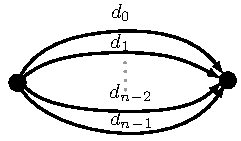
\includegraphics{distances}
\end{center}
Since the process we describe is periodic, we chose any interval of $P$ unit of time.
Describing the messages going through the two contention points during such an interval
completely define the periodic process. We call the representation of the interval
of time in the first contention point the \emph{first period} and the \emph{second period}
for the second contention point.

An \emph{offset} of a message is a choice of time at which it arrives
at the first contention point. Let us consider a message $i$
of offset $o_i$, it uses the interval of time $[i]_1 = \{ (o_i + t) \mod P \mid 0 \leq t < \tau \}$ in the first period and $[i]_2 = \{ (d_i + o_i + t) \mod P \mid 0 \leq t < \tau \}$ in the second period. We say that two messages $i$ and $j$ collide if either $[i]_1 \cap [j]_1 \neq \emptyset $ or $[i]_2 \cap [j]_2 \neq \emptyset $.

We want to send all messages, so that they are no collision in the common link.
In other word, we look for a way to send the messages without using buffering and 
hence limiting the latency to the physical length of the link. An assignment is a
choice of an offset for each message such that \emph{no pair of message collide}.
Formally, an \emph{assignment} is a function from the messages, represented by their indices in $[n]$ to their offsets in $[P]$.  

We call Periodic Message Assignment or \pma the problem we solve in this article,
which asks, given an instance of $n$ messages, a period $P$ and a size $\tau$ to find 
an assignment or to decide there is none.
\begin{center}
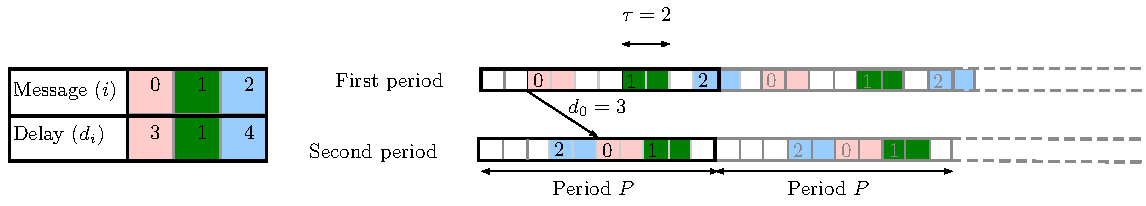
\includegraphics[scale=0.7]{instance}
\end{center}
The complexity of \pma is not known. However, we have proven that when parametrized by
$n$ the number of messages, the problem is \FPT~\cite{barth2018deterministic}.
A slight generalization, with many contention points but each message only goes through
two as in \pma is \NP-hard~\cite{barth2018deterministic} and we conjecture that \pma is \NP-hard.

To overcome the hardness, we study \pma in this article when the load of the system is small enough. The \emph{load} is defined as the number of unit of time used in a period by messages in a contention point divided by the period. Hence the load is equal to $n\tau /P$.
Our aim is to prove that for small load, there is \emph{always} an assignment and that it can be found by a polynomial time algorithm.


\section{Greedy Algorithms for Large Messages}

In this section, we study the case of large messages. When modelizing real problems,
it is relevant to have $\tau > 1$ when the transmission time is large with regard to
the delay.


A partial assignment is a function defined from a subset $S$ of $[n]$ to $[P]$.
We say that a message in $S$ is \emph{scheduled} (by $A$), and a message not in $S$ is \emph{unscheduled}. We will only consider partial assignments such that no pair of messages of $S$ collide. We denote assignment and partial assignment by $A$. If $A$ has domain 
$S$, and $i \notin S$, we define the extension of $A$ to $i$ by $v$, denoted by $A(i \rightarrow v)$, the function defined as $A$ on $S$ and such that $A(i) = v$.


All presented algorithms build the assignment incrementally, by growing the size of the domain of a partial assignment. Moreover, the algorithm of this section are greedy since once an offset is chosen for a message, it is never changed.


\subsection{First fit}


Assume that for some partial assignment $A$, the message $i$ has offset $t$: it uses all times from $t$ to $t + \tau -1$ in the first period. If a message $j$ is scheduled with some offset $t'$ before $t$, then the last time it uses in the first period is $t'+\tau-1$ and it should be less than $t$, which implies that $t' \leq t- \tau + 1$. If $t'$ is sent after $t$, to avoid collision, it should be larger or equal to $t+ \tau$. Hence the message $i$ forbid $2\tau -1$ positions for messages still not scheduled becaus eof tis use of time in the first period. The same reasonning can be done for the second period, wich again forbid $2\tau -1$ offsets. Hence, if $|S|$ messages are already scheduled, then $|S|(4\tau -2)$ offsets are forbidden for the remaining messages. Note that this is an
upper bound on the number of forbidden offsets, the same offset can be forbidden because
of a message on the first and also on the second period.

We can thus define $Fo(A)$, the maximum number of forbidden offsets when 
extending $A$. Formally, assume $A$ is defined over $S$ and $j\notin S$, 
it is the maximum over all values of $d_j$, of $|\left\{ v \in [P] \mid A(i \rightarrow v) \text{ has no collision }\right\}|$. The previous paragraph shows that $Fo(A)$ is always bounded by $(4 \tau -2)|S|$. 


The first algorithm deals with the route in the order they are given:  for each unscheduled route it tests all offsets from $0$ to $P-1$ until one do not create a collision with the current assignment.
We call this algorithm \emph{First Fit}. Remark that if $Fo(A) < P$, then whatever the delay of the route we want to extend $A$ with, it is possible to find an offset. Since $Fo(A) \leq (4 \tau -2)|S|$ and $|S| < n$, First Fit (or any greedy algorithm) will always succed 
when $(4 \tau -2)n \leq P$, that is when $ n\tau /P \leq 1/4$.
It turns out that First Fit always create compact assignments (as defined in~\cite{barth2018deterministic}), that is a message is always next to another one in one of the two period. Hence, we can prove a better bound on $Fo(A)$, when $A$ is built by First Fit, which
implies the following therem.

\begin{theorem}
First Fit always solves \pma positively on instances of load less than $1/3$. 
\end{theorem}
\begin{proof}
To prove the theorem, it is enough to prove that $Fo(A) \leq |S|(3\tau -1) + \tau -1$. 
We prove that by induction on the size of $S$. For $S = 1$, it is clear since a single
message forbid at most $(3\tau -1) + \tau -1 = 4\tau-2$ offsets. Now, assume $Fo(A) \leq |S|(3\tau -1) + \tau -1$ and consider a route $i \notin S$ such that First Fit builds $A(i \rightarrow v )$. By definition, choosing $v-1$ as offset creates a collision, w.l.o.g. 
say it is a collision on the first period. It means that there is a message between 
$v - \tau $ and $v-1$ (modulo $P$), hence all these offsets which are forbidden 
the the choice of offset of $i$ were already forbidden. It implies that only $3\tau -1$ new offsets are forbidden, that is $Fo(A(i \rightarrow v)) \leq Fo(A) + (3\tau -1)$,
which proves the induction and the theorem.
\end{proof}

\subsection{Meta-intervals}

The second method is described  in~\cite{barth2018deterministic} and achieves the same bound on the load using a different method which will also be used in the more involved algorithms
of the next section.
The idea is to restrict the possible offsets at which messages can be scheduled. It seems counter-intuitive, since it decreases artificially the number of possible offsets to schedule new messages. However, it allows to reduce the number of forbidden offsets, when the algorithm is designed accordingly. A \emph{meta-offset} is an offset of value $i\tau$,
with $i$ an integer from $0$ to $P / \tau$. We call Meta-Offset the greedy algorithm
which works as first fit, but consider only meta-offsets when scheduling new messages. 

We define $Fom(A)$ as the maximal number of meta-offsets forbidden by $A$. 
 By definition, two messages with a different meta-offset cannot collide in the first period.
Hence, $Fom(A)$ can be bounded by $3|S|$ and we obtain the following theorem.


\begin{theorem}[Proposition 3 of~\cite{barth2018deterministic} ]
Meta-Offset always solves \pma positively on instances of load less than
$1/3$.
\end{theorem}

\subsection{Tuples and meta-intervals}

We now propose a more involved family of greedy algorithms which 
solves \pma positively for larger loads. We try to combine the good properties of the two previous algorithms: the compacity of the solutions of the first one and the use of meta offsets reducing the collisions on the first period of the second one.
The idea is to schedule several routes at once, using meta-offsets, to maximize the compacity of the obtained solution. 


We first describe the algorithm which places pairs of routes and then explain quickly how we can extend it by placing tuples of routes at the same time.

We first prove a lemma which allows to assume that the period $P$ is a multiple of $\tau$, 
which makes the analysis of our algorithms much simpler and tighter. It only changes the load
from $n \tau / P$ to at most $n (\tau +1)/ P$: the difference is less than $n /P < 1/\tau$,
and is very small for large $\tau$.

\begin{lemma}
Let $I$ be an instance of \pma with $n$ messages of size $\tau$ and period $P$.
Let $m = P / \tau$. There is an instance $I'$ with $n$ messages of size $\tau'$ and period $P'= m\tau'$ such that an assignment of $I'$ can be transformed into an assignment of $I$.
\end{lemma}
\begin{proof}
Let $P = m \tau + r$ with $r \leq \tau$. We define the instance $I'$ as follows: $P' = mP$, $d_{i}' = m d_i$ and $\tau' = m \tau + r$. With this choice, we have $P' = m(m \tau + r) = m \tau'$.
Consider an assignment $A'$ of the instance $I'$.
If we let $\tau'' = m\tau$, then $A'$ is also an assignment for $I'' = (P',\tau'',(d_{0}',\dots,d_{n-1}'))$ since we only reduce the size of each message (the interval of time used in the first and second period begi at the same position but are shorter).
We then use a compactification procedure as in~\cite{barth2018deterministic}. The first message is positionned at offset zero. The first time it uses in the second period is a multiple of $m$ since its delay is by definition a multiple of $m$. Then all the other messages are translated to the left until there is a collision (remove increasing values from all offsets but the offset of the first message). It guarantees that some message is in contact with the first one,  which implies that its offset is a multiple of $m$. This procedure can be repeated until we get some solution $A''$ to $I''$, and by induction it is proven that all positions of messages in the first and second period are multiple of $m$. Hence, if we define $A$ as $A(i) = A''(i)/m$, we obtain an assignment of $I$.
\end{proof}


We are interested in the remainder modulo $\tau$ of the delays of each message.
We write $d_i = d_{i}'\tau + r_i$ and assume the messages are sorted by increasing $r_i$.
A \emph{compact pair} is a pair of messages $(i,j)$ such that we can put them
next to each other in the second period using meta-offsets.
Say that $i < j$, hence $r_i \leq r_j$ we denote by $g$ the gap between the two messages,
that we define by $d_{i}' = g + 1 + d_{j}' \mod P/\tau$. We require that $g \neq 0$ so that
there are no collision in the first period if we schedule these two messages such that the difference of their offsets is the gap. 

Faire une dessin représentant le gap, la différence des restes et la paire compacte.

\begin{lemma}\label{lemma:pair_find}
Given $3$ messages, two of them always form a compact pair. 
\end{lemma}
\begin{proof}
If the first two messages or the first and the third message form a compact pair,
then we are done. If not, then by definition $d_{1}' = 1 + d_{2}' = 1 + d_{3}'$. Hence, the messages $2$ and $3$ form a compact pair of gap $1$.
\end{proof}

We call \emph{Compact Pairs} the following greedy algorithm. From the $n$ routes in order
of increasing $r_i$, we build a sequence of at least $n/3$ compact pairs using Lemma~\ref{lemma:pair_find}. Then they are scheduled in order using meta-offsets only. When, for some compact pair, there is no more possible meta offset, or there are no more compact pairs, the remaining messages are scheduled as in Meta Offset. The analysis of the algorithm relies on the evaluation of $Fom(A)$, for the 
partial assignments produced during the first and the second phase of the algorithm. More precisely, one should evaluate the number of forbidden offsets when scheduling compact pairs, that we denote by $Fom_2(A)$ and then $Fom_(A)$. The compact pairs, only forbid $3$
offsets in the second periods instead of four if the two messages are scheduled independently, which explains the improvement from Meta Offset. We first give a simple lemma justified by Figure~\ref{}, which allows to bound this number.

\begin{lemma}\label{lemma:pair_forbid}
The position of a scheduled compact pair in the second period forbid at most four meta offsets to schedule another compact pair formed by messages with larger remainders modulo $\tau$.
\end{lemma}


\begin{theorem}
Compact Pairs always solves \pma positively on instances of load less than
$3/8$.
\end{theorem}
\begin{proof}
Let us denote by $n_2$ the number of compact pairs scheduled in the algorithm.
If we want to schedule a new pair, the position of the $2n_2$ messages on the first
period forbid $4n_2$ offsets for a compact pair. Indeed, each scheduled message can collide
with each of the two message which form a compact pair. On the second period, we can use Lemma~\ref{lemma:pair_forbid} to bound the number of forbiden offsets by $4n_2$. 
Hence, we have established that at the end of the first phase, the partial solution $A$
satisfies $Fom_2(A) \leq 8n_2$. This first phase continue while there is possible offsets for compact pairs, which is the case when $Fom_2(A) \leq m$, that is while $n_2 \leq m/8$.
In the second phase, a compact pair forbid $3$ meta offsets in the 
second period and $2$ in the first. Hence, if we let $n_1$ be the number of messages scheduled in the second phase to give the assignment $A$, we have $Fom(A) \leq n_2*5 + n_1*3.$. 
The algorithm can always schedule messages when $Fom(A)$ is less than $m$, thus
$$ n_2*5 + n_1*3 \geq m$$
$$ n_1 \geq \frac{8m - 5m }{24}$$
$$n_1 \geq \frac{1}{8}$$

The number of routes scheduled is thus at least $2n_2 + n_1$,
which is $\frac{3}{8}m$. Remark that we need to be able to schedule two third of the messages as compact pairs, which is possible by Lemma~\ref{lemma:pair_find}.Hence,  an assignment is always produced if the load is less then $\frac{3}{8}$.
\end{proof}

The algorithm can be improved by forming compact tuples instead of compact pairs.
A compact $k$-tuple is a sequence of messages $i_1,\dots,i_k$ with $r_{i_1},\dots,r_{i_k}$  increasing, for which meta offsets can be chosen so that  there are no collision and
the messages in the second period follows in order $i_1,\dots,i_k$ at a distance less than $\tau$.

Dessin d'une paire compacte et d'untriplet compact et de comment ils se gênent.

The algorithms \emph{Compact k-tuples} works by scheduling compact $k$-uples
using meta offsets while possible, then scheduling compact $k-1$-uples and so on until $k=1$.
The theorem we give is obtained for $k=10$, but taking arbitrary large $k$ and using better
bounds on $Fom(A)$ do not seem to allow for load better than $41/100$ and only work for large $n$.

Evaluate how large should be $n$.

\begin{theorem}
Compact $10$-uples always solves \pma positively on instances of load less than
$4/10$, for instance with $n$ large enough.
\end{theorem}
\begin{proof}
We use two facts, which generalizes Lemma~\ref{lemma:pair_find} and~\ref{lemma:pair_forbid} to prove this theorem:
\begin{itemize}
\item Given $ k^3/3$ messages, one can build from them a compact $k$-tuple. 
\item A $k$-tuples forbid $k+j+1$ offsets in the second period when scheduling a 
$j$-tuple. If the remainder of the messages in the $j$-tuples are larger than in the 
$k$-tuples, it forbids $k+j$ messages only.
\end{itemize}

The first fact garantees there are compact $k$-tuples, if there are enough messages.
The second one allows to estimate how many $j$-tuple for $i$ equal $k$ down to $1$
can be scheduled by bounding $Fom_j(A)$, the number of forbiden meta offsets 
when placing $j$-tuple in the algorithm.
A numerical computation of the number of each kind of tuples scheduled shows that 
$Fom(A) < m$ for any partial solution built by the algorithm when the load is less than $4/10$.
\end{proof}



\subsection{Experimental results}

Results better in practice, the worst case is different from the 
average case.
The algorithms to test:
\begin{itemize}
	\item first fit
	\item choix randomisé de l'offset possible
	\item meta offset
	\item heuristic to build super compact assignment: among the compact assignments
possible, chose the one which minimizes the number of forbidden offsets
	\item algo avec les paires tant que c'est possible, si on a le temps
	\item FPT pour avoir la borne absolue
\end{itemize}

On représente le taux de succès en fonction de la charge. On peut faire
pour des paquets de taille $1000$ et une période de $100 000$ comme ça on
peut faire une charge par pas de 1 pour cent. On peut sans doute commencer
le graphique à 33 pour cent car la plupart des algos sont garantis marcher 
tout le temps en dessous. 
Meilleure idée ? 

Quality of the results partially explained by the average analysis done later.
 

\section{Reduction from large message to message of size one}

\subsection{Reduction without buffering}

Methode avec perte de load d'un facteur $1/2$ : considère 
des messages deux fois plus gros et on se sert d'un trick de décalage pour 
pour que tous les $d_i$ soient bien alignés.  
Utile pour les arguments qui montrent qu'en moyenne on
réussit pour une charge $1$, se transfert pour charge $1$.


\subsection{Reduction  using buffering}

Possibility of buffering the route during a time $b$: change $d_i$ to $d_i + b$. 
Form of tradeoff between latency (more latency implies smaller message size implies
solution with higher load).


All messages are buffered enough time so that their $d_i$ have the same
remainder modulo $\tau$. It costs at most $\tau$ of buffering (which is not
good in our application but not horrible either). We can choose the longest 
route as reference, hence that route cost zero. 
If all distances are of $d_i$ a multiple of $\tau$, we have an
easy reduction to the case of $\tau = 1$, by dividing all values by $\tau$.


We can do the same kind of transformation by buffering all 
messages, so that the $d_i$ are multiples of $\tau / k$. The cost in term
of latency would be $\tau / k$ but the reduction yields message of size $k$.
For small size of messages, it is easy to get better algorithm (in particular for $\tau =1$
as we show in the next section).
\begin{theorem}
Compact pairs on instances with $\tau =2$ always solves \pma positively on instances of load less than $4/9$.
\end{theorem}
\begin{proof}
We assume w.l.o.g that there are less message with even $d_i$ than odd $d_i$.
We schedule compact pairs of messages with even $d_i$, then we schedule single message with 
even $d_i$. The worst case is when there is the same number of the two type of messages.
The number of forbidden offsets for $n$ scheduled messages is bounded by 
$$ n/2 (1 + 3/2) + n/2(1 + 1). $$

Hence, we can always schedule messages when $n \leq (4/9)m$.

\end{proof}


If we want to optimise for the average latency, we win a factor of two as we now explain.

Define the average buffer time for a choice of reference: B(t). 
If we sum the $B(t)$ for $t=0$ to $\tau-1$, the contribution of each message 
will be $\sum_{i=0}^{\tau-1} i$. Hence, the sum of the $B(t)$ is 
$n P (P-1)/2$. There is at least one term of the sum less than the average,
hence there is a $t_0$ such that $B(t_0) \leq n (\tau-1)/2$. In other word, the average
delay for the message is less than $\tau/2$.



Finally, solution with no buffering but which doubles the load. 



\section{Going Above Load of 1/2 for messages of size one}


Expliquer que le genre de méthode utilisé dépend de toutes les routes,
impossible en streaming, impossible de rajouter une route avec les mêmes garanties.
Peut-être possible de faire un swap avec une autre route ?


%There are easier cases, all routes are distinct or all routes are the same. There is a solution for load $1$ in these two cases. With two distinct values, solution for load almost one. Insert a figure here, showing solutions
%for these cases.
We  give a method which always finds a solution for load $1/2 + \epsilon$.


To go above $1/2$ of load, we use a two-pass algorithm. In the second pass, a greedy algorithm is used 
to place a subsets of the routes, selected because they have less conflicts with the already placed 
routes. The first pass is not greedy, since we allow to change fixed route, but we could us a greedy first
pass or even a single pass greedy algorithm to go over $1/2$. However, the proofs are much harder and 
the $\epsilon$ for which they hold is much smaller.

\begin{definition}
The potential of a route of shift $s$ in a partial solution (whether fixed or not in the partial solution),
is the number of integers $i \in [P]$ such that $i$ is used in the forward window and $i+s \mod P$ is used in the backward window. We denote by Pot(S) the sum of potentials of the routes in the partial solution S.
\end{definition} 


\begin{definition}
The potential of a position $i$ of the forward window, for a partial solution, is the number of routes of shift $s$ such that $i+s$ is used in the partial solution. 
\end{definition}

The potentials of the positions satisfy the following simple invariant.
\begin{lemma}\label{lemma:inv}
The sum of potentials of all positions of the forward window in a partial solution of size $k$ is $nk$.  
\end{lemma}

We then link Pot(S) to the potential of the positions in the forward window.
\begin{lemma}\label{lemma:pot_pos}
The sum of potentials of all used positions in the forward window in a partial solution S is equal to Pot(S).  
\end{lemma}
 

We now describe the algorithm to solve our problem with load $1/2 + \epsilon$. The first pass assign routes in any
greedy manner, until it cannot assign some route anymore. Then, it applies some procedure described later which 
remove a route from the solution and add anther one. If at some point this procedure fails, it stops.
When this algorithm stops, it can be shown that the potential of the obtained partial solution is larger
than some value. Then, we select $R$ the set of the $\epsilon P$ routes of largest potential. The routes in $R$ and in the partial solution are removed, then the free routes not in $R$ are added to the partial solution and 
finally the route in $R$ are added, using any greedy algorithm.

\subsection{Swap and potential improvement}


Let $S$ be some partial solution of size $k$ and let $r$ be a free route of shift $s$. 
Assume that $r$ cannot be used to extend $S$. The swap operation is the following: 
select a free position $p$, remove the route of position $p+s$ in the forward window 
of $S$ and add $r$ at position $p$ in the forward window. We denote this operation by $Swap(r,p,S)$.

\begin{lemma}
Let $S$ be some partial solution of size $k$ and let $r$ be a free route of shift $s$. 
If $r$ cannot be used to extend $S$, then either $Pot(Swap(r,p,S)) > Pot(S)$ or 
$Pot(S) \geq kn/2$.
\end{lemma}

\begin{proof}\label{swap}
The positions in the forward window can be partitionned into two part: $P_{u}$ the positions used in the forward windows and $P_{f}$ the positions unused in the forward windows.
Let us denote by $V_f$ the value of the positions in $P_f$ and by $V_u$ the potential of the positions of $P_u$. By Lemma~\ref{lemma:pot_pos}, since $P_f$ and $P_u$ partitions the positions, we have $V_f + V_u = kn$.

By hypothesis, since $r$ cannot be placed, for all $p \in P_{f}$, $p+s$ is used in the backward window. We now define a function $F$ which associates to $p \in P_{f}$ the position $p'$ such that there is a route $r'$ in $S$ placed at $p'$ in the forward window and at $p+s$ in the backward window. The function $F$ is an injection from $P_{f}$ to $P_u$. Rmeark now that if we compare $Swap(r,p,S)$ to $S$, on the backward window nothing changes. 
Hence the potential of each position in the forward window is the same. Hence, doing the operation $Swap(r,p,S)$ add to $Pot(S)$ the potential of the position $p$ and removes the potential of position $F(p)$. 
Assume now, to prove our lemma, that for all $p$, $Pot(Swap(r,p,S)) \leq Pot(S)$. It implies that 
$V_f \leq V'_u \leq V_u$ and by Lemma~\ref{lemma:inv} we have $V_f \leq Pot(S)$.
Since $V_f + Pot(S) = kn$, we have that $Pot(S) \geq kn/2$.
\end{proof}


% 
% 
% \begin{lemma}\label{lemma:improvement}
% We assume that there are at least $P/2$ distinct routes.
% Given a partial solution $S$ of size $k\leq P/4$, such that 
% $Pot(S) = \frac{k^2n}{2P}$, there is a free route which can be placed at some position, adding $kn/P+1$ of value.
% \end{lemma}
% \begin{proof}
% 
% By Lemma~\ref{lemma:pot_pos}, the sum of the potential of the used positions in $S_{k}$ is $Pot(S) = k^2n/2P$. Since there are $k$ used positions, their average value is $kn/2P$.
% By Lemma~\ref{lemma:inv}, the sum of potentials is $kn$, hence 
% the average value of a position is $kn/P$. As a consequence of these two facts, there is a free position of value more than the average $kn/P$.
% TODO: we can assume that the average value of the free positions is larger
% than the average value of the used ones -> chose the parameter optimaly.
% 
% 
% Since there are at least $P/2$ disctinct routes, and $k$ are used,
% there are at least $P/2 -k$ free distinct routes. Since $k \leq P/4$,
% there are more distinct routes avalaible than fixed route, hence any free position can be occupied by at least one free route.
%  
% Hence we can always put a route on the free position of potential $\frac{kn}{P}$. Moreover, fixing a route add one to its own potential, which increases the potential of the partial solution by $kn/P+1$.
% \end{proof}
% 
% Encore pas bon, on doit s'arrêter à $P/4$ et pas $P/2$
% pour garantir de toujours trouver une route qui couvre, 
% ce qui donne un gain de seulement $1/64$.


\subsection{Analysis of the Algorithm}


We give an analysis of the algorithm, showing that it works for some value
of $\epsilon$. We will later show that some refinments of this algorithm: a better selection of the 
values added in the second step, the possibility to repeat the first step to guarantee a higher potential
yields a better $\epsilon$.


\begin{theorem}
The two-pass algorithm solves positively our problem with load $1/2 + 1/16$.
\end{theorem}

\begin{proof}
 The first pass of the algorithm guarantes that we obtain a partial solution 
 $S$ of size $k$ such that $Pot(S) \geq kn/2$ by Lemma~\ref{lemma:swap}. 
 Moreover, $k \geq P/2$ since one can always place $P/2$ routes with a greedy algorithm.
 
At the end of the first pass, we have a potential of at least $Pn/4$ and we select the $\epsilon P$ routes of largest potential. They must be of potential at least $2\epsilon P, 2\epsilon P +2,\dots ,4\epsilon P$.
Sort all routes by decreasing potential and assume that the previous condition is not met, that is the $i$th route in order of potential is of potential less than $4\epsilon P - 2i$. The potential of a single route is bounded by $P/2$ since each placed route contribute at most one to its potential. Therefore, the first
$i$ routes are of potential at most $P/2$ and the following ones of potential at most $4\epsilon P - 2i$. Therefore the potential is less than $iP/2 + (4\epsilon P - 2i) (n -i)$. This function is decreasing for $i \leq \epsilon P$, hence the potential should be less than $4\epsilon P n$.
 
 For the algorithm to succeed, we want the potential to be larger than $4\epsilon P n$ so that the condition on the routes of largest potential is met.
Hence we must satisfy the following equation:
 $$Pn/4 \geq 4\epsilon P n.$$
 $$ \epsilon \leq 1/16.$$
\end{proof}


Pour améliorer les résultats on peut répéter l'algo de swap une fois qu'on a obtenu 
au moins $(1/2 + \epsilon)P$ routes placées, pour obtenir $n^2/2$ en potentiel. 
On doit alors avoir $n^2/2 \geq 4\epsilon P n$, ce qui donne $\epsilon \leq 1/14$.
Si on veut pousser la technique plus loin, il faut améliorer la borne sur le potentiel.
Au lieu de prendre les $\epsilon P$ plus grandes routes, on prend pour $i$ de $1$
à $\epsilon P$ la route de plus petit potentiel supérieur à $2 \epsilon P$ et 
pour qu'elle existe, il suffit que le potentiel soit supérieur à $2\epsilon P (n -i)$.
À vérifier, si à un moment tout est de potentiel $2 \epsilon P$ au moins, alors 
c'est facile de conclure. On obtient alors $\epsilon \leq 1/6$, ce qui donne un algo
dès que la charge est inférieure à $2/3$.

Autre possibilité, améliorer le potentiel en obtenant plus que la moyenne, en jouant notemment sur la symétrie Backward et Forward.

Expliquer les nombreuses raisons pourquoi ça marche mieux en pratique.




\section{Algorithms for random instances}

\paragraph{$\tau = 1$}

We analyze the following process, called \textbf{Uniform Greedy} or UG.
For each element in order, chose one admissible position
uniformly at random. We analyze the probability that Uniform Greedy
solve the problem, averaged over all possible instances. 
It turns out that this probability, for a fixed load strictly less than one goes to zero when $m$ grows. 

Définir l'ensemble des solutions de taille $n$ parmi $m$.
\begin{theorem}
Given an instance of size $n$ uniformly at random UG
produces a solution uniformly at random or fail.
\end{theorem}
\begin{proof}
Regarder mes notes partielles pour compléter ça.
\end{proof}

Let us denote by $P(m,n)$ the probability that UG fails at the $n_th$
steps assuming it has not failed before.

\begin{theorem}
We have $$P(m,n) = \frac{\binom{n}{2n-m}}{\binom{m}{n}}.$$
In particular, $P(m,n) \leq f(\lambda)^m$, where $f(\lambda) < 1$.
\end{theorem}
\begin{proof}
Probability independent of the shift of the $n$ element, can say it is $0$.
It is the probability that two sets of size $n$ in $[m]$ are of union $[m]$.
It is the same as the probability that it contains a given set of size $m-n$.
Could find an asymptotic online.
\end{proof}

Can we make the same argument for a deterministic algorithm?
The not average version of the argument is the previous proof.

Show that we can find a solution for load $1/2 - \epsilon$, even for large 
$\tau$ if $n$ is large enough, using the trnasformation without buffering.

\section{Experimental results for $\tau = 1$}


\section{Lower bounds}

Example/family of examples for which some greedy alg fail.
Example/family of examples with a given load such that there are no feasible solution.

\bibliographystyle{ieeetr}
 \bibliography{Sources}

\end{document}
